\begin{savequote}[8cm]
Alles Gescheite ist schon gedacht worden.\\
Man muss nur versuchen, es noch einmal zu denken.

All intelligent thoughts have already been thought;\\
what is necessary is only to try to think them again.
  \qauthor{--- Johann Wolfgang von Goethe \cite{von_goethe_wilhelm_1829}}
\end{savequote}

\chapter{\label{ch:2-litreview}Background}

\minitoc
 This chapter summarises the main aspects of the tropical circulation and the lin defines a monsoon. 
\section{The tropical circulation and the global monsoon}\label{sq:bk_tropics}

Tropical climate is characterized by the strong incoming solar insolation year-round that makes the tropics the warmest region of the planet. 
The strong solar insolation and surface temperature are also associated with strong evaporative fluxes and ultimately convection. 
 These characteristics largely influence the tropical circulation which, to a first order, can be described through the zonal and meridional circulations known as the Hadley and Walker cells. 
 
 


\begin{figure}
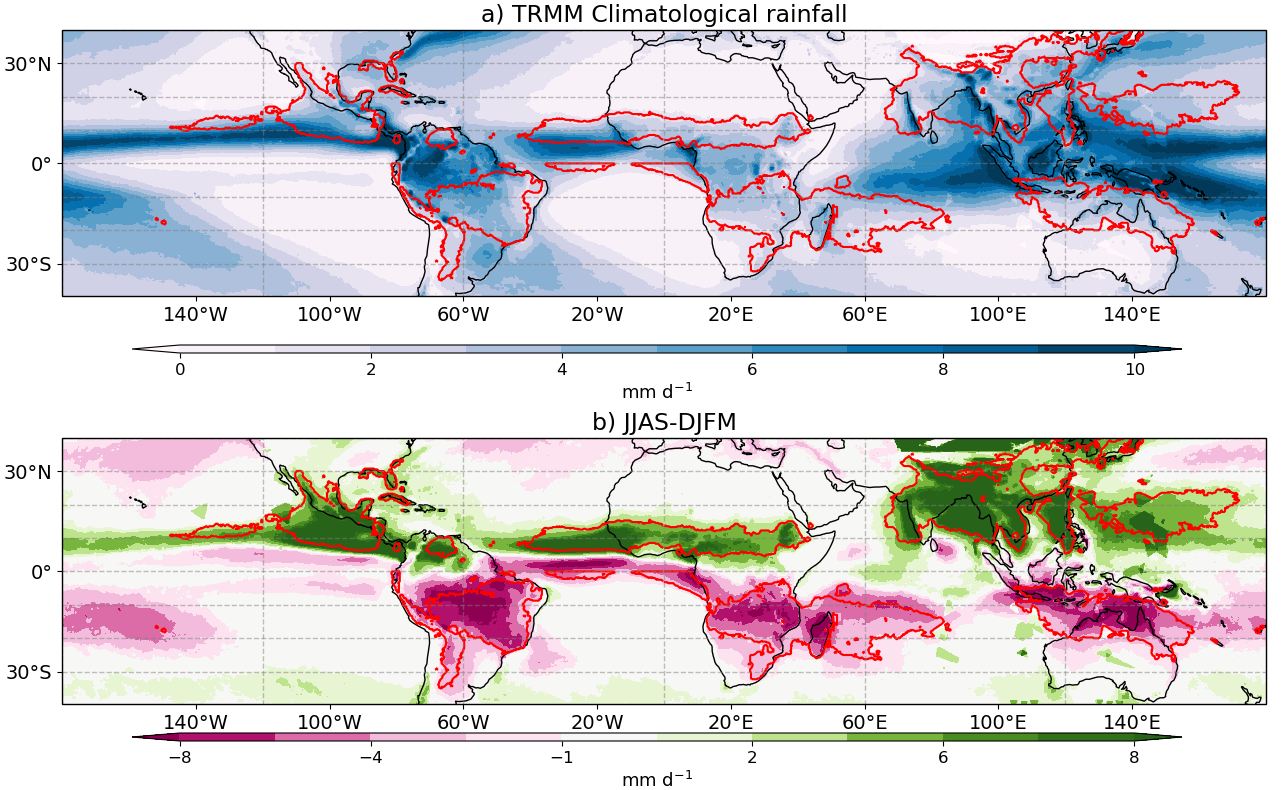
\includegraphics[width=\linewidth]{figures/trmmclima.png}
\caption{a) Climatological mean annual rainfall rates in the tropics in the TRMM dataset (1999-2018). b) The mean rainfall rate difference between boreal summer (JJAS) and austral summer (DJFM). The red contours highlight the regions where the summer rainfall amount accounts for more than 55\% of the total annual rainfall accumulation. }
\label{fig:monsoon}
\end{figure}

The Inter-tropical Convergence Zone (ITCZ) is a band of precipitation that migrates meridionally with the seasons and is arguably one of the most relevant features of tropical climate. The ITCZ is characterized by a strong convergent flow in the low levels and a strong divergent flow at upper levels. 

The global monsoon refers to the those regions of the planet where more than 70\% of the total annual rainfall falls during the summer season \citep{zhou2016,wang2017}.
Figure \ref{fig:monsoon} shows the global monsoon as depicted by the TRMM dataset. By this definition, the majority of the regions over land between 5 and 10 degrees away from the equator are part of the global monsoon.

A regional monsoon, such as the Indian Monsoon, is then a subset of the global monsoon with unique regional characteristics that shape this monsoon different to other regional monsoons in terms of the seasonality, the strength and the dynamics. 

The American Monsoon System is then the regional monsoon that is located in the subtropics of North and South America. 
\section{The American Monsoon System}\label{sq:bk_ams}

The AMS is typically subdivided into the North and South American monsoon systems \citep{vera2006}.
The North American Monsoon is the main source of rainfall in south-western North America, extending north from central-west Mexico into the southwestern United States \citep{adams1997,stensrud1997,vera2006}.
 The seasonal cycle of rainfall in the North American Monsoon is characterised by a wet July-August-September season and significantly drier conditions during the rest of the year \citep{adams1997}.
A key aspect of this monsoon is the moisture advected by the low-level flow from the Gulf of California and the East Pacific Ocean and to a lesser extent the moisture mixed in the mid-troposphere from the Caribbean Sea and Gulf of Mexico \citep[e.g][]{stensrud1997,pascale2016,ordonez2019}.
%%

The South American Monsoon is a primary source of precipitation for South America, especially in the Amazon region \citep{gan2004,vera2006,jones2013}.
During austral summer (DJF), monsoon rainfall accounts for over 60\% of the total annual precipitation in the Amazon \citep{gan2004,marengo2012}, whereas
austral winter rainfall accounts for less than 5\% of the total annual rainfall \citep{vera2006}.
In the central Amazon, convective precipitation is observed from early October but the main rainy season extends from December to April \citep{machado2004,adams2013}, whereas convection in southeastern Brazil and Paraguay starts in November and peaks in January and February \citep{marengo2001,nieto2011}. 

A bimodal regime characterises the seasonal cycle of precipitation in southern Mexico, Central America and the Caribbean, most commonly known as Midsummer Drought (MSD) \citep{magana1999,gamble2008} \citep{dilley1996,amador2016,duranquesada2017}.
The seasonal cycle in these regions is characterised by two precipitation maxima, in June and September, that are separated by a drier period in July and August.
The complex interplay of sea-surface temperatures (SSTs), evaporation and moisture transport between the East Pacific Ocean and the Caribbean Sea are key for the spatial and temporal characteristics of the MSD \citep{amador2006,herrera2015,duranquesada2017,straffon2019}.

\section{El Niño Southern Oscillation: impacts to the American monsoon system}
\label{sub:diagnostic}

Beyond the chest X-ray (`plain film'), the key non-invasive imaging modalities in diagnostic cardiology are echocardiography, magnetic resonance imaging, and X-ray computed tomography, which are reviewed below.  Nuclear medicine, including positron emission tomography (PET) and single-photon emission computed tomography (SPECT), are not discussed here, as they do not play a role in the chapters to follow.

\section{Stratosphere-Troposphere Coupling in the Tropics}

\begin{figure}
\centering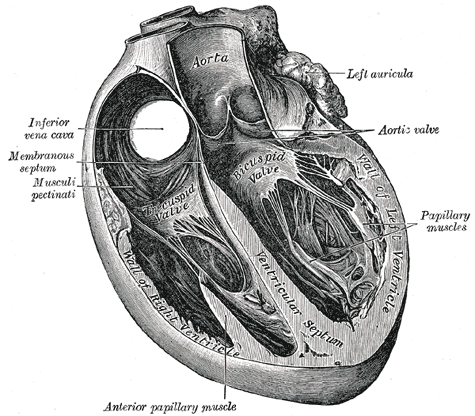
\includegraphics[width=0.7\textwidth]{figures/sample/Gray498.png} 
\caption[Four-chamber illustration of the human heart.]{Four-chamber illustration of the human heart.  Clockwise from upper-left: right atrium, left atrium, left ventricle, right ventricle.}
\label{fig:fourchamber}\end{figure}

The use of acoustic waves for medical diagnosis, inspired by naval sonar, was initially developed in the 1940s \cite{gagliardi_ultrasonography_1996}.  By 1954, the first clinically useful cardiac ultrasound -- examining motion of the mitral valve in stenosis -- was reported \cite{edler_ultrasonic_1957}.  These early scans were one-dimensional images (`A-mode'), sometimes repeated to generate a time axis (`M-mode').   The sector-scanning probe was developed in the 1970s \cite{bom_ultrasonic_1971,griffith_sector_1974}, leading to the `B-mode' that a modern cardiologist would recognise as an echocardiogram.
